\documentclass[a4paper,12pt]{extreport}

\usepackage[utf8]{inputenc}
\usepackage[T1]{fontenc}
\usepackage{mathpazo}
\usepackage{amsmath,amssymb}
\usepackage{booktabs}
\usepackage{array}
\usepackage{graphicx}
\usepackage{float}
\usepackage{xcolor}
\usepackage{geometry}
\usepackage{hyperref}
\usepackage{xurl}
\usepackage{caption}
\usepackage{enumitem}
\usepackage{listings}
\usepackage{microtype}

\graphicspath{{report_assets/}{.}}
\geometry{a4paper,left=25mm,right=20mm,top=25mm,bottom=25mm}
\hypersetup{colorlinks=true,linkcolor=black,citecolor=black,urlcolor=blue}
\captionsetup{justification=centering}
\setcounter{tocdepth}{2}
\setcounter{secnumdepth}{2}
\setlength{\parindent}{1.5em}
\setlength{\parskip}{0.4em}
\renewcommand{\arraystretch}{1.2}

\lstset{
    language=Python,
    basicstyle=\small\ttfamily,
    frame=single,
    breaklines=true,
    showstringspaces=false,
    keywordstyle=\color{blue},
    commentstyle=\color{green!45!black},
    stringstyle=\color{purple}
}

% If an image has not been uploaded yet, this macro leaves a visible frame
% containing the exact expected file name.
\newcommand{\reportfigure}[4][0.95\linewidth]{%
\begin{figure}[H]
    \centering
    \IfFileExists{#2}{%
        \includegraphics[width=#1]{#2}%
    }{%
    \IfFileExists{report_assets/#2}{%
        \includegraphics[width=#1]{report_assets/#2}%
    }{%
        \fbox{\parbox[c][6cm][c]{0.9\linewidth}{%
            \centering Expected image file:\\[0.5em]
            \texttt{\detokenize{#2}}%
        }}%
    }}
    \caption{#3}
    \label{#4}
\end{figure}
}

\begin{document}

% =============================================================================
% Cover page
% =============================================================================
\begin{titlepage}
\thispagestyle{empty}
\begin{center}
    {\large\color{red} HANOI UNIVERSITY OF SCIENCE AND TECHNOLOGY}\\[0.3cm]
    {\large\color{red} School of Information and Communications Technology}\\[0.6cm]
    \textbf{-------------------- $\ast$ --------------------}\\[1.2cm]

    \IfFileExists{hustss.png}{
        \includegraphics[width=4cm]{hustss.png}
    }{
        \fbox{\parbox[c][4cm][c]{4cm}{\centering University logo\\\texttt{hustss.png}}}
    }\\[1.2cm]

    {\fontsize{28pt}{34pt}\selectfont\textbf{PROJECT REPORT}}\\[0.8cm]

{\fontsize{20pt}{25pt}\selectfont\textbf{A FROM-SCRATCH CONVOLUTIONAL}}\\[0.15cm]
{\fontsize{20pt}{25pt}\selectfont\textbf{NEURAL NETWORK}}\\[0.4cm]

{\fontsize{18pt}{23pt}\selectfont FOR 16$\times$16 HANDWRITTEN CHARACTER}\\[0.15cm]
{\fontsize{18pt}{23pt}\selectfont RECOGNITION}\\[0.4cm]

{\fontsize{16pt}{20pt}\selectfont WITH USER CORRECTION COLLECTION}
\end{center}

\vfill
\begin{center}
\large
\begin{tabular}{@{}ll@{}}
    \textbf{Supervisor:} & Dr. Nguyen Ba Ngoc \\
    \textbf{Student:} & Mai Vu Hoang \\
    \textbf{Student ID:} & 202416695
\end{tabular}
\end{center}

\vfill
\begin{center}
    {\large Ha Noi, \the\year}
\end{center}
\end{titlepage}

\pagenumbering{roman}
\chapter*{Abstract}
\addcontentsline{toc}{chapter}{Abstract}
This project presents a lightweight Convolutional Neural Network (CNN) implemented from scratch with NumPy for recognizing handwritten characters on binary $16\times16$ grids. The system uses a prepared 47-class EMNIST Balanced dataset containing digits, uppercase letters, and 11 distinct lowercase classes. To reduce overfitting and computation, the current architecture preserves two convolutional blocks but reduces the dense hidden layer from 128 to 64 units, resulting in 40,687 trainable parameters. Training includes best-checkpoint selection, early stopping, and adaptive learning-rate decay based on validation-loss plateaus.

The final Dense-64 benchmark uses a practical 14,100-image balanced dataset budget so that both model training and controlled parameter tuning can be completed on Kaggle CPU. On the balanced 1,410-image test set, the saved model reaches 79.43\% accuracy, 0.8031 macro-precision, 0.7943 macro-recall, and 0.7918 macro-F1. A separate 10-epoch run with the same principal configuration reaches 80.43\% test accuracy in the dataset-size experiment. The strongest errors occur between visually similar low-resolution classes such as F/f, 0/O, 1/I/L, 2/Z, and 9/q/g. Spatial-shift testing shows that centering is important for mouse-drawn input: random shifts reduce accuracy to 52.41\%, while recentering restores it to 78.16\%.

\noindent\textbf{Keywords:} optical character recognition, handwritten character recognition, convolutional neural network, EMNIST, NumPy, low-resolution images.

\tableofcontents
\clearpage
\pagenumbering{arabic}

% =============================================================================
\chapter{Introduction}

\section{Problem Statement}
Optical Character Recognition (OCR) converts visual symbols into machine-readable labels. Although modern OCR systems often use deep architectures and optimized tensor frameworks, this project studies a constrained educational setting: recognizing one character from a binary $16\times16$ image using a CNN whose layers, forward propagation, backward propagation, and parameter updates are manually implemented with NumPy. CNN-based document recognition is historically grounded in LeNet-style systems for handwritten and document images~\cite{lecun1998gradient}.

The low resolution creates substantial ambiguity. Curves, stroke intersections, and gaps may occupy only one or two pixels. Consequently, classes such as 0/O, 1/I/L, 2/Z, 5/S, 9/q, and F/f can become visually similar. The challenge is not only to obtain reasonable aggregate accuracy, but also to understand which classes fail, how position affects prediction, and whether the architecture is appropriately sized for the data.

Let an input be $x\in\{0,255\}^{16\times16}$ and let the label space contain $K=47$ classes. The model learns
\begin{equation}
f_{\theta}:\mathbb{R}^{16\times16}\rightarrow\mathbb{P}(\mathcal{Y}),
\end{equation}
where $\theta$ denotes trainable filters, weights, and biases, and $\mathbb{P}(\mathcal{Y})$ is a probability distribution over the 47 labels. The implementation must run on CPU without PyTorch, TensorFlow, pretrained weights, or library-provided neural-network layers.

\section{Objectives}
The project has the following objectives:
\begin{itemize}[leftmargin=2em]
    \item implement Conv2D, ReLU, MaxPool2D, Flatten, Dense, Softmax, cross-entropy, and backpropagation from scratch;
    \item train on a class-balanced subset of EMNIST Balanced;
    \item design a CNN whose spatial dimensions remain valid for a $16\times16$ input;
    \item reduce overfitting through a smaller classifier, learning-rate decay, best-checkpoint saving, and early stopping;
    \item evaluate overall and per-class performance;
    \item compare dataset size, initial learning rate, learning-rate decay, and padding;
    \item quantify sensitivity to spatial displacement and the benefit of centering;
    \item demonstrate an interactive drawing interface and a user-correction collection workflow.
\end{itemize}

% =============================================================================
\chapter{Theoretical Background}
\label{sec:theoretical-background}

\section{Problem Formulation}

\subsection*{Data Space and Static Optimization}
The stored input space is $\mathcal{X}=\{0,255\}^{16\times16}$. The label set $\mathcal{Y}$ contains ten digits, 26 uppercase letters, and 11 lowercase letters. Given a training set $D_{\mathrm{train}}=\{(x_i,y_i)\}_{i=1}^{N}$, the objective is
\begin{equation}
\theta^{*}=\arg\min_{\theta}\frac{1}{N}\sum_{i=1}^{N}
\mathcal{L}(f_{\theta}(x_i),y_i).
\end{equation}
For one-hot target $y_i$ and predicted probability $\hat{y}_i$, categorical cross-entropy is
\begin{equation}
\mathcal{L}(\hat{y}_i,y_i)=-\sum_{j=1}^{K}y_{i,j}\log(\hat{y}_{i,j}+10^{-9}).
\end{equation}

\subsection*{Correction Collection}
The system includes an interactive correction workflow for collecting additional labelled handwriting after deployment. The detailed interface demonstration and feedback mechanism are described later in Section~\ref{sec:interactive-demo}. In this report, feedback is treated as a data-collection feature rather than as a measured accuracy improvement.

\section{CNN Operations for Low-Resolution Binary Images}

\subsection*{Convolution and Padding}
For input tensor $X$ and filter $W_f$, the convolution output is
\begin{equation}
Z_{i,j,f}=\sum_{u=0}^{k-1}\sum_{v=0}^{k-1}\sum_{c=0}^{C-1}
X_{i+u,j+v,c}W_{u,v,c,f}+b_f.
\end{equation}
The reported benchmark model uses $3\times3$ filters, stride one, and one-pixel zero padding. Padding preserves the spatial dimensions before pooling, which is particularly important because the input is only $16\times16$.

\subsection*{Activation, Pooling, and Classification}
The ReLU activation is $\operatorname{ReLU}(z)=\max(0,z)$. A non-overlapping $2\times2$ max-pooling operation then halves width and height. Two pooling layers therefore transform the spatial resolution as $16\rightarrow8\rightarrow4$, leaving a $4\times4$ representation rather than collapsing the image too aggressively.

After flattening, a 64-unit dense layer combines the extracted features. The output layer produces 47 logits, which Softmax converts to probabilities:
\begin{equation}
p_j=\frac{\exp(z_j-\max(z))}{\sum_{k=1}^{K}\exp(z_k-\max(z))}.
\end{equation}
Subtracting the maximum logit improves numerical stability.

\subsection*{Optimization and Evaluation}
Combining Softmax and cross-entropy gives the output gradient $p-y_{\mathrm{one-hot}}$. Parameters are updated after each image:
\begin{equation}
\theta\leftarrow\theta-\eta\nabla_{\theta}\mathcal{L}.
\end{equation}
The effective batch size is one. Accuracy measures overall correctness, while macro-precision, macro-recall, and macro-F1 weight every class equally. A confusion matrix reveals systematic visual ambiguities that aggregate accuracy cannot show.

Weights use He initialization:
\begin{equation}
W\sim\mathcal{N}\left(0,\frac{2}{n_{\mathrm{in}}}\right),
\end{equation}
which is suitable for ReLU networks.

% =============================================================================
\chapter{Methodology and System Implementation}
\label{sec:methodology}

This chapter describes direct dataset loading, balanced partitioning, the current Dense-64 CNN, its training controls, and the local drawing interface.

\section{Data Loading and Dataset Partitioning}
The training program directly loads \texttt{data/emnist\_47\_classes\_16x16.npz}, which is derived from the EMNIST handwritten-character dataset~\cite{cohen2017emnist}. No resizing, thresholding, rotation, or augmentation is performed by \texttt{train.py}. The file contains \texttt{X} with shape $(47{,}000,16,16)$ and \texttt{y} with shape $(47{,}000,)$. Images are binary \texttt{uint8} matrices with 0 as background and 255 as foreground.

The 47 classes comprise 0--9, A--Z, and the lowercase classes a, b, d, e, f, g, h, n, q, r, and t. Unicode labels are sorted and encoded as indices 0--46 for the Softmax output.

To keep the from-scratch CPU implementation practical while leaving enough time for parameter tuning, the program selects an equal number per class under a 14,100-image base budget:
\begin{equation}
n_{\mathrm{class}}=\left\lfloor\frac{14{,}100}{47}\right\rfloor=300.
\end{equation}
The balanced total is therefore 14,100. Each class contributes 240 base training images, 30 validation images, and 30 test images, producing base partitions of 11,280, 1,410, and 1,410 images. Optional correction samples, when present, are appended only to the training partition. Validation and test partitions remain unchanged.

\reportfigure{class_distribution.png}
{Balanced class distribution in the base training, validation, and test partitions.}
{fig:class-distribution}

\section{Custom CNN Architecture for 16x16 Inputs}
The architecture is deliberately shallow. Two convolutional blocks are sufficient to build local and compound stroke features, while two pooling operations leave a $4\times4$ grid. Reducing the dense hidden layer from 128 to 64 lowers the parameter count from 76,527 to 40,687, a reduction of approximately 46.8\%, without changing convolutional feature extraction.

\subsection*{Input Normalization}
Pixels are mapped from $[0,255]$ to $[-0.5,0.5]$ inside the forward pass:
\begin{equation}
x'=\frac{x}{255}-0.5.
\end{equation}
This numerical scaling is not dataset preprocessing; it is part of model computation.

\subsection*{First Convolutional Block}
Conv1 applies 16 filters of size $3\times3$ with padding one, producing $16\times16\times16$. ReLU introduces nonlinearity and $2\times2$ max pooling reduces the tensor to $8\times8\times16$.

\subsection*{Second Convolutional Block}
Conv2 applies 32 filters of size $3\times3$ with padding one, producing $8\times8\times32$. After ReLU and pooling, the output is $4\times4\times32$.

\subsection*{Fully Connected Classifier}
The pooled tensor is flattened into 512 values. Dense1 maps $512\rightarrow64$, followed by ReLU. Dense2 maps $64\rightarrow47$, followed by Softmax.

\begin{table}[H]
\centering
\caption{Current CNN architecture for $16\times16$ inputs.}
\label{tab:architecture}
\resizebox{\textwidth}{!}{%
\begin{tabular}{llllr}
\toprule
Layer & Input & Configuration & Output & Parameters \\
\midrule
Input & $16\times16$ & Normalize & $16\times16\times1$ & 0 \\
Conv1 & $16\times16\times1$ & 16 filters, $3\times3$, pad 1 & $16\times16\times16$ & 160 \\
ReLU1 + Pool1 & $16\times16\times16$ & ReLU, pool $2\times2$ & $8\times8\times16$ & 0 \\
Conv2 & $8\times8\times16$ & 32 filters, $3\times3$, pad 1 & $8\times8\times32$ & 4,640 \\
ReLU2 + Pool2 & $8\times8\times32$ & ReLU, pool $2\times2$ & $4\times4\times32$ & 0 \\
Flatten & $4\times4\times32$ & Flatten & 512 & 0 \\
Dense1 & 512 & 64 units + ReLU & 64 & 32,832 \\
Dense2 & 64 & 47 units & 47 & 3,055 \\
Softmax & 47 & Probability normalization & 47 & 0 \\
\midrule
\multicolumn{4}{r}{\textbf{Total}} & \textbf{40,687} \\
\bottomrule
\end{tabular}}
\end{table}

\subsection*{Weight Initialization and Loss Calculation}
Convolution and dense weights use He initialization, which is designed for rectifier networks~\cite{he2015}; biases start at zero. Cross-entropy adds $10^{-9}$ before the logarithm to avoid $\log(0)$.

\subsection*{Training Controls}
The initial learning rate is 0.004. Whenever validation loss fails to improve for one epoch, the learning rate is multiplied by 0.5 down to a minimum of 0.001. Whenever validation loss improves by at least $10^{-4}$, the model is saved as the new best checkpoint. Early stopping uses patience four and cannot trigger before epoch 7. After training, the best checkpoint rather than the final in-memory state is loaded for test evaluation.

% =============================================================================
\chapter{Experiments and Evaluation}

\section{Dataset and Baseline Analysis}
The exported class-distribution plot confirms equal base support for all 47 labels. The current baseline uses 14,100 selected EMNIST images: 240 training, 30 validation, and 30 test samples per class. Optional correction samples are not used to alter validation or test support, and no separate feedback-ablation claim is made.

The training curves show steady learning across seven epochs. Training accuracy increases from 70.19\% to 89.72\%, while validation accuracy increases from 68.01\% to 78.79\%. Validation loss reaches its best value of 0.6400 at epoch 7. After validation loss worsens at epoch 6, the scheduler reduces the learning rate from 0.004 to 0.002; the following epoch becomes the best checkpoint. The final train--validation accuracy gap is 10.92 percentage points, indicating moderate overfitting rather than a complete failure to generalize.

\reportfigure{training_curves.png}
{Training and validation curves reconstructed from the final Dense-64 training log.}
{fig:training-curves}

\begin{table}[H]
\centering
\caption{Final Dense-64 baseline results for the 14,100-image benchmark.}
\label{tab:baseline-results}
\begin{tabular}{lr}
\toprule
Metric & Result \\
\midrule
Test loss & 0.6597 \\
Test accuracy & 79.43\% \\
Macro-precision & 0.8031 \\
Macro-recall & 0.7943 \\
Macro-F1 & 0.7918 \\
Mean confidence & 84.32\% \\
Mean inference time & 42.60 ms/image \\
Parameters & 40,687 \\
Model file size & 329,058 bytes \\
\bottomrule
\end{tabular}
\end{table}

\begin{table}[H]
\centering
\caption{Final training-log summary.}
\label{tab:training-summary}
\begin{tabular}{lr}
\toprule
Item & Value \\
\midrule
Completed epochs & 7 \\
Best checkpoint epoch & 7 \\
Best validation loss & 0.6400 \\
Best validation accuracy & 78.79\% \\
Learning-rate reductions & 1 \\
Final learning rate & 0.002 \\
Total training time & 12,506.86 s \\
\bottomrule
\end{tabular}
\end{table}

\section{Controlled Model Experiments}

\subsection*{Effect of Dataset Size}
The dataset-size experiment trains separate Dense-64 models for up to 10 epochs using an initial learning rate of 0.004, validation-loss-based decay, and padding one. The comparison uses class-balanced sizes that are exact multiples of 47: 2,350, 4,700, 7,050, 9,400, and 14,100 images. Accuracy generally improves as the subset grows, from 65.11\% to 80.43\%. The slight dip at 9,400 images is plausible because each setting is trained only once and uses a different balanced subset and optimization trajectory; repeated runs would be needed to determine whether the difference is statistically reliable.

\begin{table}[H]
\centering
\caption{Effect of dataset size for the Dense-64 CNN.}
\label{tab:sample-size}
\begin{tabular}{rrrrr}
\toprule
Images & Accuracy & Macro-F1 & Test loss & Runtime (s) \\
\midrule
2,350 & 65.11\% & 0.6354 & 1.2424 & 2,174.78 \\
4,700 & 72.77\% & 0.7214 & 0.9153 & 4,358.67 \\
7,050 & 78.87\% & 0.7862 & 0.7868 & 6,526.67 \\
9,400 & 76.91\% & 0.7681 & 0.8219 & 8,685.15 \\
14,100 & 80.43\% & 0.8031 & 0.6483 & 11,330.73 \\
\bottomrule
\end{tabular}
\end{table}

\reportfigure{sample_size_comparison.png}
{Dataset-size comparison for the Dense-64 CNN.}
{fig:sample-size}

The 80.43\% result in this experiment and the saved baseline accuracy of 79.43\% come from separate training runs with different training horizons. The distributed baseline is trained for seven epochs and selects epoch 7, whereas the 14,100-image experiment is allowed ten epochs and selects epoch 8. Therefore, 79.43\% is reported as the performance of the distributed model file, while 80.43\% is reported as the best controlled experimental run.

\subsection*{Effect of Learning Rate}
Each value in this experiment is used as the initial learning rate and is then controlled by the same reduce-on-plateau schedule. The control subset contains 7,050 balanced images so that learning-rate conclusions are closer to the final 14,100-image run while still remaining practical to execute. The best control result is obtained with an initial learning rate of 0.004, while 0.012 is less stable and produces the weakest result.

\begin{table}[H]
\centering
\caption{Initial learning-rate comparison for the Dense-64 CNN.}
\label{tab:learning-rate}
\begin{tabular}{rrrr}
\toprule
Learning rate & Accuracy & Macro-F1 & Test loss \\
\midrule
0.002 & 76.88\% & 0.7697 & 0.7732 \\
0.004 & 78.87\% & 0.7862 & 0.7868 \\
0.008 & 75.74\% & 0.7501 & 0.7748 \\
0.012 & 73.19\% & 0.7223 & 0.9119 \\
\bottomrule
\end{tabular}
\end{table}

\reportfigure{learning_rate_comparison.png}
{Initial learning-rate comparison for the Dense-64 CNN.}
{fig:learning-rate}

\subsection*{Effect of Learning-Rate Decay}
The evaluation suite also isolates the learning-rate schedule itself by comparing reduce-on-plateau with a fixed learning rate. Both runs use the same 7,050-image control subset, initial learning rate 0.004, padding one, Dense-64 classifier, best-checkpoint selection, and early-stopping rule. Reduce-on-plateau reaches 78.87\% accuracy, compared with 74.04\% for the fixed-rate run, an improvement of 4.83 percentage points. This supports retaining adaptive decay in the final training configuration.

\begin{table}[H]
\centering
\caption{Learning-rate decay comparison for the Dense-64 CNN.}
\label{tab:lr-decay}
\begin{tabular}{lrrrr}
\toprule
Schedule & Accuracy & Macro-F1 & Test loss & LR reductions \\
\midrule
Reduce on plateau & 78.87\% & 0.7862 & 0.7868 & 2 \\
Fixed learning rate & 74.04\% & 0.7264 & 0.8449 & 0 \\
\bottomrule
\end{tabular}
\end{table}

\reportfigure{lr_decay_comparison.png}
{Comparison between fixed learning rate and validation-loss-based learning-rate decay.}
{fig:lr-decay}

\subsection*{Effect of Padding}
The padding experiment compares the same Dense-64 model with and without one-pixel convolution padding on the 7,050-image control subset. Padding one improves test accuracy from 73.33\% to 78.87\% and macro-F1 from 0.7311 to 0.7862. It preserves border information but increases the parameter count from 16,111 to 40,687 and the measured inference time from 23.26 to 42.56 ms/image. For this low-resolution task, the 5.53-point accuracy gain justifies the additional computation, so padding one is retained in the final model.

\begin{table}[H]
\centering
\caption{Padding comparison for the Dense-64 CNN.}
\label{tab:padding}
\begin{tabular}{rrrrr}
\toprule
Padding & Accuracy & Macro-F1 & Parameters & Inference \\
 & & & & (ms/image) \\
\midrule
0 & 73.33\% & 0.7311 & 16,111 & 23.26 \\
1 & 78.87\% & 0.7862 & 40,687 & 42.56 \\
\bottomrule
\end{tabular}
\end{table}

\reportfigure{padding_comparison.png}
{Padding comparison for the Dense-64 CNN.}
{fig:padding}

\section{Robustness and Error Analysis}

\subsection*{Confusion Matrix and Per-Class Performance}
The dominant confusions are visually plausible for $16\times16$ binary characters. The largest errors are F/f (17 images), 1/I (14), 0/O (11), q/9 (11), L/I (9), L/1 (8), and 2/Z (7). The weakest F1 scores are for 1 (0.3333), q (0.3600), F (0.4231), L (0.4681), I (0.5570), 0 (0.5902), f (0.6000), and g (0.6071). The strongest classes include X (0.9677), 3 (0.9667), W (0.9375), h (0.9355), and C (0.9355). These errors show that remaining failures are concentrated in character pairs with nearly identical strokes at low resolution.

\reportfigure[0.9\linewidth]{confusion_matrix_counts.png}
{Confusion matrix counts for the final Dense-64 benchmark.}
{fig:confusion-counts}

\reportfigure[0.9\linewidth]{confusion_matrix_normalized.png}
{Normalized confusion matrix for the final Dense-64 model.}
{fig:confusion}

\reportfigure{f1_by_class.png}
{F1 score by class for the final Dense-64 model.}
{fig:f1-by-class}

\reportfigure[0.9\linewidth]{misclassified_examples.png}
{Misclassified examples with true label, prediction, and confidence.}
{fig:misclassified}

\subsection*{Spatial Robustness}
Random shifts of up to two pixels reduce test accuracy from 79.43\% to 52.41\%. Cropping and centering the shifted image restores accuracy to 78.16\%. This result supports the centering operation used in the drawing interface, because mouse-drawn characters are rarely placed in exactly the same position as dataset samples.

\begin{table}[H]
\centering
\caption{Spatial-robustness results for the final Dense-64 model.}
\label{tab:robustness}
\begin{tabular}{lrr}
\toprule
Condition & Accuracy & Mean loss \\
\midrule
Original & 79.43\% & 0.6597 \\
Random shift $[-2,2]$ & 52.41\% & 2.1317 \\
Shifted then centered & 78.16\% & 0.7234 \\
\bottomrule
\end{tabular}
\end{table}

\reportfigure{shift_robustness.png}
{Robustness to random shifts and subsequent centering.}
{fig:shift-robustness}

\section{Interactive Recognition System and Demo}
\label{sec:interactive-demo}
The GUI loads class labels and architecture metadata from the saved model. A user draws with the left mouse button, erases with the right button, and requests a prediction. The interface is designed around the same $16\times16$ binary representation used by the training data: each displayed square corresponds to one input pixel, white cells are encoded as 255, and black cells are encoded as 0. This makes the demo faithful to the actual model input instead of using a higher-resolution drawing that would require extra preprocessing.

The model file can be loaded directly from \texttt{models/emnist\_47\_brain.npz} or extracted automatically from \texttt{artifacts/cnn\_evaluation\_results.zip}. This allows the interface to run locally without the EMNIST dataset after training has completed.

\subsection*{Demo Case Analysis}
Figure~\ref{fig:gui-demo-correct} and Figure~\ref{fig:gui-demo-feedback} show the two main interaction paths of the deployed interface. The first case demonstrates normal inference when the model prediction is accepted. The second case demonstrates the correction workflow when the displayed prediction is not the intended label.

\begin{figure}[H]
    \centering
    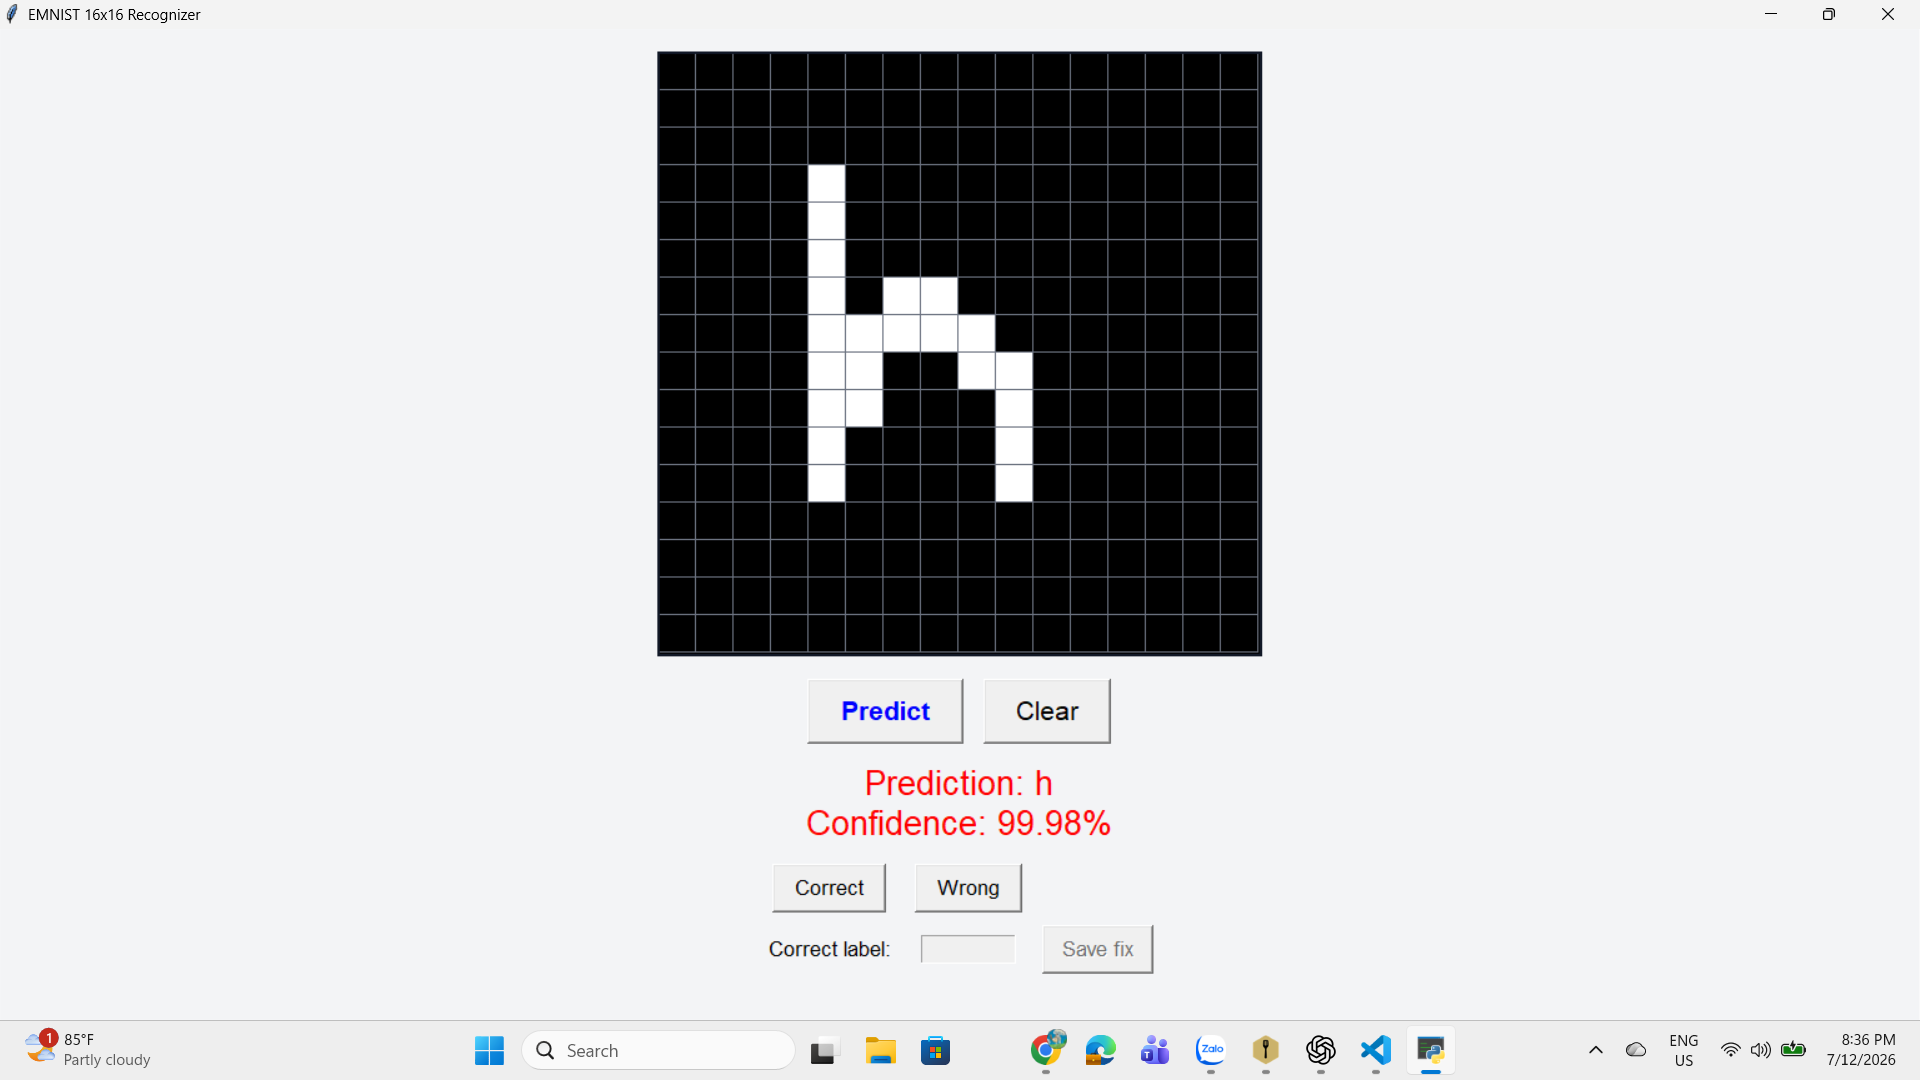
\includegraphics[width=0.95\linewidth]{gui_demo_correct.png}
    \caption{Correct-prediction demo. The user draws a lowercase \texttt{h}; the CNN predicts \texttt{h} with 99.98\% confidence, so the sample does not need to be saved as feedback.}
    \label{fig:gui-demo-correct}
\end{figure}

\begin{figure}[H]
    \centering
    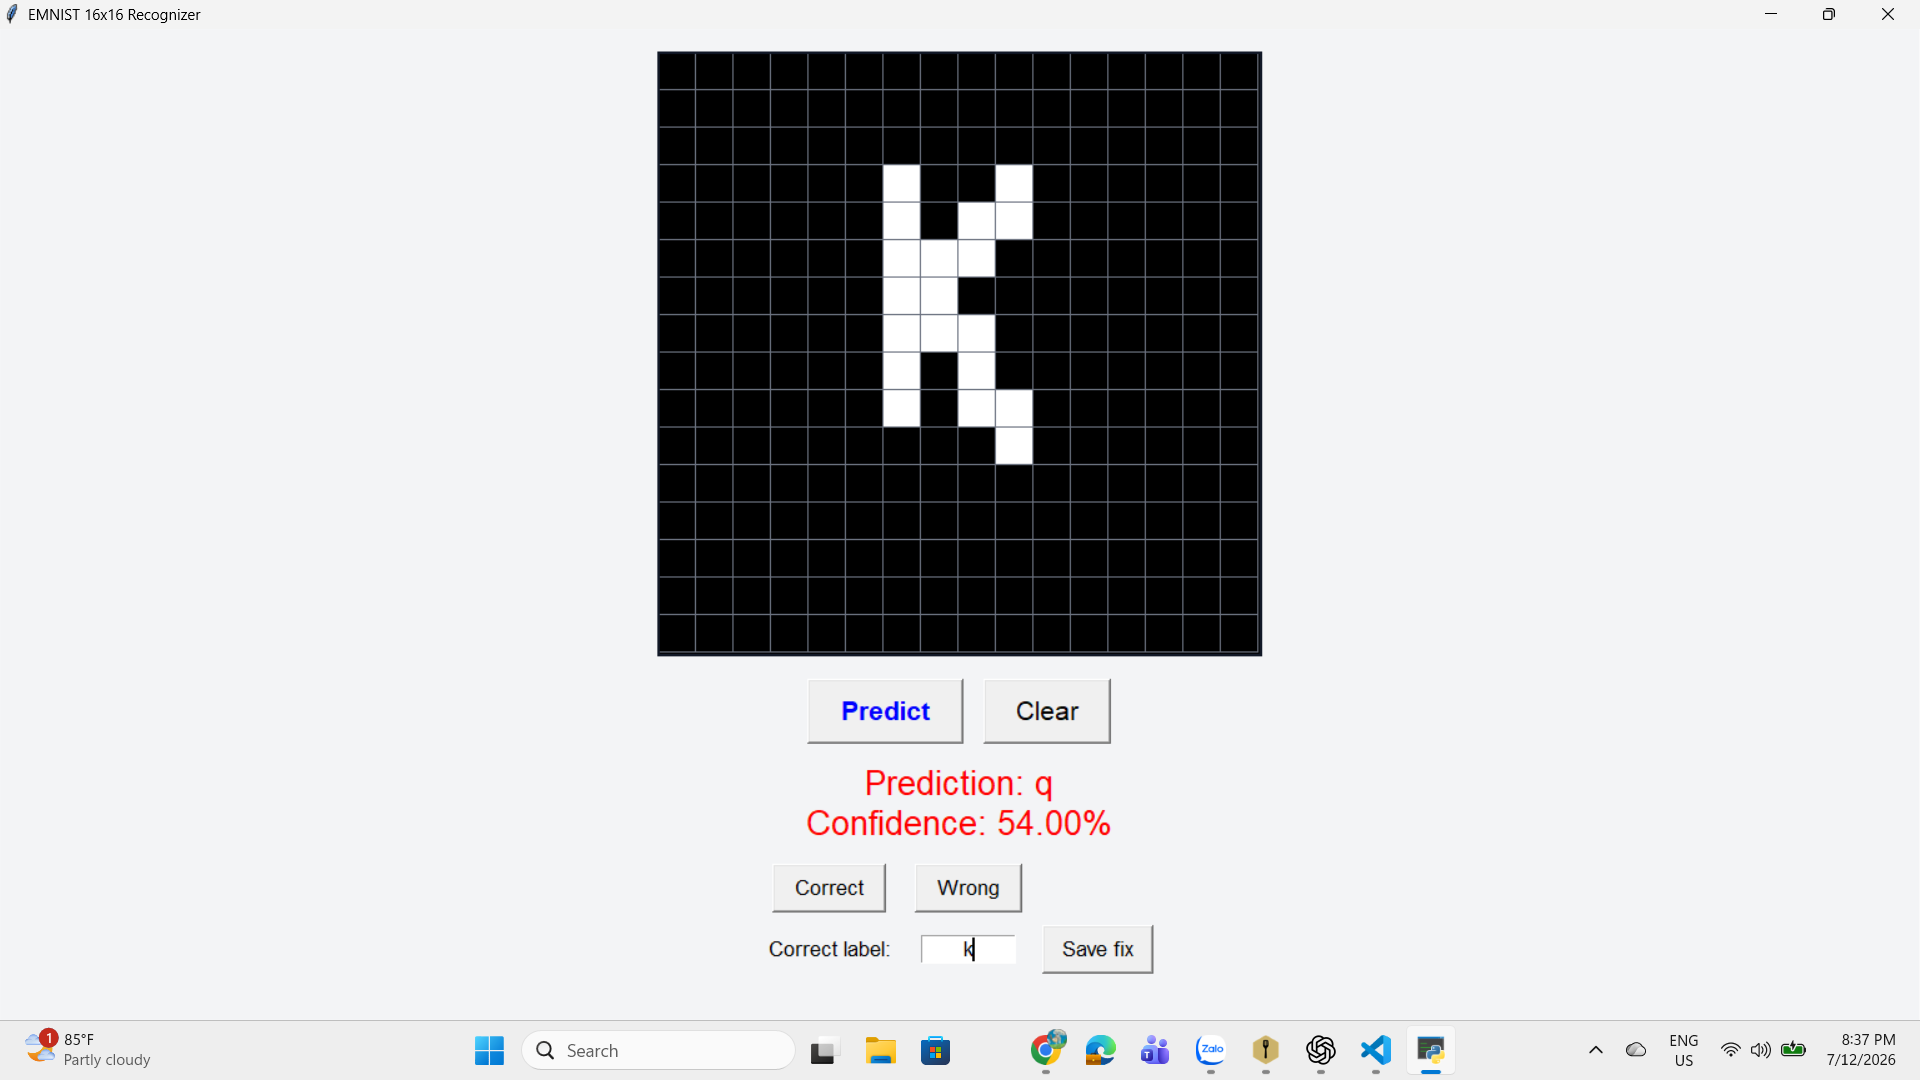
\includegraphics[width=0.95\linewidth]{gui_demo_feedback.png}
    \caption{Incorrect-prediction demo. The CNN predicts \texttt{q} with 54.00\% confidence, and the correction field is enabled so that the user can provide the intended label.}
    \label{fig:gui-demo-feedback}
\end{figure}

\begin{table}[H]
\centering
\caption{Interpretation of the two GUI demonstration cases.}
\label{tab:gui-demo-analysis}
\begin{tabular}{p{0.24\textwidth}p{0.33\textwidth}p{0.33\textwidth}}
\toprule
Demo case & Observation & System behavior \\
\midrule
Correct prediction & The drawn lowercase \texttt{h} is predicted as \texttt{h} with very high confidence. & The user can press \texttt{Correct}; no new training sample is written because the model output already matches the intended label. \\
Incorrect prediction & The model predicts \texttt{q} with lower confidence, indicating ambiguity in the $16\times16$ drawing. & The user presses \texttt{Wrong}, enters a corrected label, and saves the sample only if the label belongs to the supported 47-class label set. \\
\bottomrule
\end{tabular}
\end{table}

\subsection*{User Feedback Mechanism}
The feedback mechanism is intentionally separated from evaluation. After pressing \texttt{Predict}, the current drawing is first centered by cropping the non-empty bounding box and placing it in the middle of a new $16\times16$ grid. The centered image is passed to the saved CNN, which returns a predicted label and a confidence score. The GUI then asks the user whether the prediction is correct. Figure~\ref{fig:gui-demo-correct} shows the normal successful path: the user can press \texttt{Correct}, and no extra training sample is saved.

If the prediction is wrong, the user selects \texttt{Wrong}. The correction field is then enabled, as shown in Figure~\ref{fig:gui-demo-feedback}, and the user must enter the true label. The label is case-sensitive and must belong to the 47 supported classes: digits, uppercase letters, and the supported lowercase letters. For example, uppercase \texttt{K} is valid, while lowercase \texttt{k} is rejected because it is not part of the selected 47-class EMNIST label set. Invalid labels are rejected before saving.

When a valid correction is submitted, the GUI appends one sample to \texttt{data/user\_feedback\_47\_classes\_16x16.npz}. The saved arrays have the same format as the training data: \texttt{X} stores binary images with shape $(N,16,16)$ and \texttt{y} stores integer class labels. The CNN weights are not updated immediately inside the GUI. Instead, the correction file is used as additional training data the next time \texttt{train.py} is run. This design keeps inference fast and simple while still allowing new user handwriting to be collected for later retraining.

During retraining, correction samples are appended only to the training partition. Validation and test partitions remain based on the original balanced EMNIST split, so reported benchmark accuracy is not inflated by user-provided examples. The current report therefore does not claim a measured performance gain from feedback; it only demonstrates a practical mechanism for collecting future data.

\reportfigure{feature_maps.png}
{Representative feature maps from the final Dense-64 model.}
{fig:feature-maps}

% =============================================================================
\chapter{Conclusions}

\subsection*{Key Findings}
The current architecture is structurally appropriate for $16\times16$ inputs. Two padded convolutional blocks preserve edge information, while two pooling operations leave a $4\times4$ feature grid. Reducing the dense hidden layer to 64 keeps the saved model at 40,687 parameters while reaching 79.43\% test accuracy and 0.7918 macro-F1 on a balanced 47-class test set. The corresponding 10-epoch, 14,100-image controlled run reaches 80.43\%, confirming that the selected configuration is capable of approximately 80\% accuracy when given a slightly longer training horizon.

Best-checkpoint saving prevents a weaker epoch from replacing a stronger validation state. In the final training log, the best validation loss occurs at epoch 7. The adaptive learning-rate schedule reduces the learning rate after validation-loss plateaus, and the controlled schedule comparison confirms that decay improves generalization over a fixed learning rate at the same initial value.

\subsection*{Practical Implications}
The results identify several practical design choices. First, explicit centering is essential for mouse-drawn input because it recovers most of the accuracy lost under random spatial shifts. Second, an initial learning rate of 0.004 outperforms 0.002, 0.008, and 0.012 on the 7,050-image control subset. Third, validation-loss-based decay improves accuracy by 4.83 percentage points over keeping 0.004 fixed. Fourth, padding one produces a substantial accuracy gain over padding zero, although it increases parameters and inference time. The saved-model metadata and ZIP-loading workflow make local deployment straightforward. The demo interface also provides a practical route for collecting additional handwriting, although no improvement claim is made without an independent evaluation.

\subsection*{Limitations and Future Work}
The evaluation uses one configured random seed and one balanced split per run, so the observed differences have no confidence intervals. The fixed test support of 30 images per class is useful for balance but remains limited. Training is slow because convolution and backpropagation are implemented with Python and NumPy loops rather than optimized deep-learning kernels. The model does not use training-time augmentation, L2 regularization, dropout, or a separate user-level holdout set. Future work may add repeated-seed evaluation, manual mini-batch vectorization, lightweight training-only augmentation, probability calibration, and a controlled feedback study.

% =============================================================================
\appendix
\chapter{Reproducibility}
The current model and evaluation suite are executed with:
\begin{lstlisting}
python train.py
python run_all_evaluations.py
\end{lstlisting}

For evaluation-only reruns with an existing trained model, execute:
\begin{lstlisting}
python run_all_evaluations.py
\end{lstlisting}
The resulting \texttt{artifacts/cnn\_evaluation\_results.zip} contains the saved model, CSV/JSON metrics, report figures, and source files needed to reproduce the reported evaluation. Report figures are stored in \texttt{report\_assets/}. For Overleaf submission, either upload the \texttt{report\_assets} folder with the same structure or upload the PNG files directly next to \texttt{main.tex}; the report uses short figure names such as \texttt{training\_curves.png}, \texttt{sample\_size\_comparison.png}, \texttt{lr\_decay\_comparison.png}, \texttt{gui\_demo\_correct.png}, and \texttt{gui\_demo\_feedback.png}.

\begin{thebibliography}{9}
\addcontentsline{toc}{chapter}{References}
\bibitem{cohen2017emnist}
G. Cohen, S. Afshar, J. Tapson, and A. van Schaik,
``EMNIST: an extension of MNIST to handwritten letters,''
\textit{2017 International Joint Conference on Neural Networks (IJCNN)}, pp. 2921--2926, 2017.
doi: \href{https://doi.org/10.1109/IJCNN.2017.7966217}{10.1109/IJCNN.2017.7966217}.

\bibitem{lecun1998gradient}
Y. LeCun, L. Bottou, Y. Bengio, and P. Haffner,
``Gradient-based learning applied to document recognition,''
\textit{Proceedings of the IEEE}, vol. 86, no. 11, pp. 2278--2324, Nov. 1998.
doi: \href{https://doi.org/10.1109/5.726791}{10.1109/5.726791}.

\bibitem{he2015}
K. He, X. Zhang, S. Ren, and J. Sun,
``Delving deep into rectifiers: Surpassing human-level performance on ImageNet classification,''
\textit{Proceedings of the IEEE International Conference on Computer Vision (ICCV)}, pp. 1026--1034, 2015.
doi: \href{https://doi.org/10.1109/ICCV.2015.123}{10.1109/ICCV.2015.123}.
\end{thebibliography}

\end{document}
